The optical properties of a non-square interdiffused quantum well
depend on the band structure which can be found by using some
existing models, such as the envelop function approximation,
pseudopotential method, the tight-binding model and the effective
bond-orbital model. We use the envelop function approximation
because of the computationally simplicity and enough accuracy for
describing phenomena occurring on a length scale large compared with
the unit cell of the crystal. The envelop function for the
z-direction can be obtained by solving the Schrodinger-like equation
shown below.
\begin{equation}\label{schrodinger}
    \frac{-h^2}{2} \frac{d}{dz} \frac{1}{m_\perp^*(z)} \frac{d\varphi(z)}{dz}
    +V(z)\varphi(z)
        = E\varphi(z)
\end{equation}
where $m_\perp(z)$ is the effective mass of the
conduction band or valence band. $V(z)$ is the position-dependent
potential energy of the conduction band heavy hole valence band
or light hole valence band, which can be determined by Equation
\ref{V_c}-\ref{V_LH}, respectively.
This differential equation is solved using the
finite-difference method (FDM) with appropriate boundary conditions.
Usually we consider the quantum well contained in a large box along
the z-direction with the boundary condition $\varphi=0$ at the
boundaries of the box.
\begin{equation}\label{V_c}
    V_c(z)
        = Q_c Eg(z) - (1-Q_c)S_\perp(z)
\end{equation}

\begin{equation}\label{V_HH}
    V_{HH}(z)
        = (1-Q_c)[Eg(z) - S_\perp(z)] + S_\parallel(z)
\end{equation}

\begin{eqnarray}\label{V_LH}
    V_{LH}(z)&=& (1-Q_c)[Eg(z) - S_\perp(z)] \notag\\
    && +0.5[S_\parallel(z) + \Delta_0(z)] \notag\\
    && -0.5 \sqrt{9S_\parallel^2(z)-2S_\parallel^2(z)\Delta_0(z)+\Delta_0^2(z)}
\end{eqnarray}

The calculation of the potential energy has take consideration
the strain effect of the quantum well materials by
Equation \ref{S_perp}-\ref{epsilon}.
All the material parameters for the numerical calculation can be obtained
from Table \ref{parametertable} by \cite{table}.
\begin{equation}\label{S_perp}
    S_\perp(z)
        = -2a_v(z)[1-\frac{C_{12}(z)}{C_{11}(z)}] \epsilon(z)
\end{equation}
\begin{equation}\label{S_parallel}
    S_\parallel(z)
        = -b(z)[1+\frac{2C_{12}(z)}{C_{11}(z)}] \epsilon(z)
\end{equation}
\begin{equation}\label{a_v}
    a_v(z)
        = -\frac{1}{3}[C_{11}(z)+2C_{12}(z)] \frac{dEg}{dp}(z)
\end{equation}
\begin{equation}\label{epsilon}
    \epsilon(z)
        = \frac{a_{InP}(z)-a(z)}{a(z)}
\end{equation}

\begin{table*}[!t]
    \renewcommand{\arraystretch}{1.3}
    \caption{Material parameters for InGaAsP used in numerical calculation
        at room temperature (300K) of Quantum Wells structures}
    \centering
    \label{parametertable}
    \begin{tabular}{llll}
        \hline
        \hline
        Symbol & Parameter & $In_{x}Ga_{1-x}As_{y}P_{1-y}$ & Unit\\
        \hline
        $Q_c:Q_v$ & Band offset splitting ratio & $0.6:0.4$ & $-$\\
        $E_g(z)$ & Energy bandgap & $1.35-1.17y+0.668(1-x)-0.069y(1-x)+0.18y^2$ & eV\\
                                  && $+0.03(1-x)y^2+0.758(1-x)^2-0.322y(1-x)^2$ &\\
        $\Delta_0(z)$ & Spin-orbit splitting & $0.34(1-x)y+0.43xy+0.10(1-x)(1-y)+0.10x(1-y)$ & eV\\
        $m_e$ & Electron mass & $0.91095\times10{-30}$ & kg\\
        $m_c^*(z)$ & Electron effective mass & $0.0632(1-x)y+0.0213xy+0.17(1-x)(1-y)+0.077x(1-y)$ & $m_e$\\
        $m_{\perp HH}^*(z)$ & Heavy hole effective mass & $0.5(1-x)y+0.41xy+0.54(1-x)(1-y)+0.12x(1-y)$ & $m_e$\\
                            & perpendicular to QW layer &&\\
        $m_{\perp LH}^*(z)$ & Light hole effective mass & $0.088(1-x)y+0.024xy+0.16(1-x)(1-y)+0.12x(1-y)$ & $m_e$\\
                            & perpendicular to QW layer &&\\
        $m_{\parallel HH}^*(z)$ & Heavy hole effective mass & $0.11(1-x)y+0.031xy+0.19(1-x)(1-y)+0.15x(1-y)$ & $m_e$\\
                                & parallel to QW layer &&\\
        $m_{\parallel LH}^*(z)$ & Light hole effective mass & $0.23(1-x)y+0.082xy+0.34(1-x)(1-y)+0.29x(1-y)$ & $m_e$\\
                                & parallel to QW layer &&\\
        $a(z)$ & Lattice constant & $0.56533(1-x)y+0.60584xy+0.54512(1-x)(1-y)+0.58688x(1-y)$ & nm\\
        $C_{11}(z)$ & Elastic stiffness constant & $11.8(1-x)y+8.329xy+14.12(1-x)(1-y)+10.22x(1-y)$ & $10^{11}dyn/cm^2$\\
        $C_{12}(z)$ & Elastic stiffness constant & $5.38(1-x)y+4.526xy+6.253(1-x)(1-y)+5.76x(1-y)$ & $10^{11}dyn/cm^2$\\
        $dE_g/dP(z)$ & Hydrostatic pressure coefficient & $11.5(1-x)y+10.0xy+11.0(1-x)(1-y)+8.5x(1-y)$ & $10^{-6}eV/bar$\\
        $b(z)$ & Shear deformation potential & $-1.7(1-x)y-1.8xy-1.5(1-x)(1-y)-2.0x(1-y)$ & eV\\
        \hline
        \hline
    \end{tabular}
\end{table*}

To show the validity of the theoretical model, I adopt the data by Nanyang
Technology University with the same method of argon plasma-induced QWI \cite{redshift}.
The layer structure of samples used in the experiment is shown in Table \ref{RedShiftSample}.
Figure \ref{ex_redshift} shows the PL spectra of one InP cap sample before plasma exposure
and after plasma exposure followed by several rapid thermal annealing (RTA) process.
The result shows that after argon plasma exposure, both the blueshift and redshift
of the bandgap can be obtained by controlling the temperature of RTA.

\begin{table}[!t]
    \renewcommand{\arraystretch}{1.3}
    \caption{The layer structure for the undoped InGaAsP/InP single quantum well}
    \centering
    \label{RedShiftSample}
    \begin{tabular}{cccc}
        \hline
        \hline
        No. & Composition & Thickness(nm) & Layer\\
        \hline
        5 & $In_{0.53}Ga_{0.47}As$ & 500 & Buffer/cap\\
        4 & InP & 500 & Barrier/cap\\
        3 & $In_{0.71}Ga_{0.29}As_{0.61}P_{0.39}$ & 3.5 & Well\\
        2 & InP & 300 & Barrier\\
        1 & InP & $-$ & substrate\\
        \hline
        \hline
    \end{tabular}
\end{table}

\begin{figure}[!t]
    \centering
    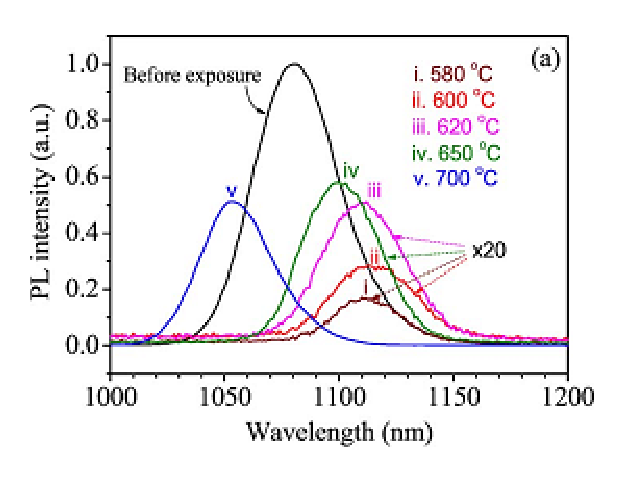
\includegraphics[width=2.5in]{fig/exp_red}
    \caption{PL spectra for one InP cap sample before plasma exposure and after plasma
        exposure followed by annealing at (i) 580$^\circ$C, (ii) 600$^\circ$C, (iii) 620$^\circ$C,
        (iv) 650$^\circ$C, (v) 700$^\circ$C.}
    \label{ex_redshift}
\end{figure}

To interpret the above observations of bandgap modification,
the wavelength shift of the interdiffused QW structure was calculated using
my theoretical model. Figure \ref{my_redshift} shows the calculated PL peak
wavelength shift as a function of group III diffusion length under different k
parameters. It can be seen that, in this QW structure, an observable redshift
can be obtained only when k$<$0.63 roughly; i.e., the group III sublattice must
interdiffuse about twice as fast as the group V sublattice.

\begin{figure}[!t]
    \centering
    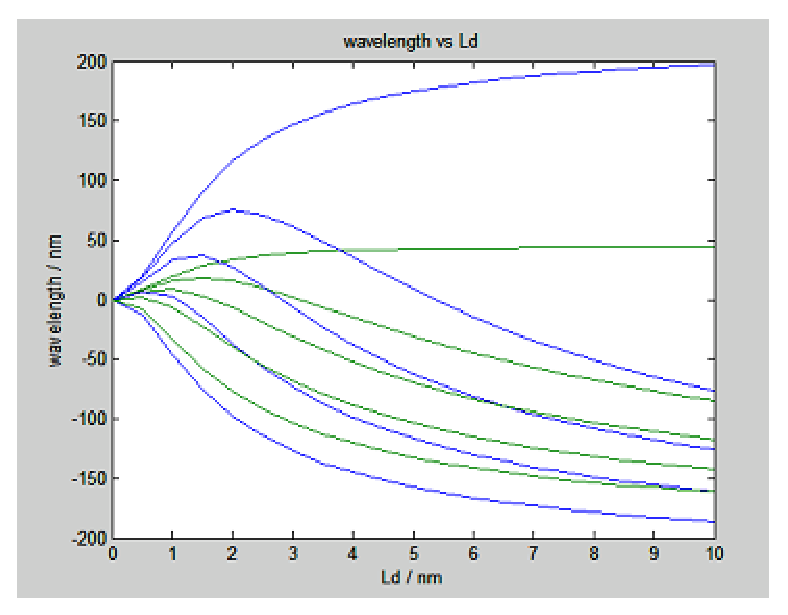
\includegraphics[width=2.5in]{fig/red}
    \caption{The calculated wavelength shift of the ground state transition
        as a function of the group III diffusion length under different k parameters.}
    \label{my_redshift}
\end{figure}
